\chapter{Facebook Integration}
\label{FBI}

\section{Introduction}
\label{FBI:introduction}
--- To be filled ---

\section{Prerequisites}
\label{FBI:settingUpProject}

Before we can use the facebook api we must perform certain prerequisite tasks.

\subsection{Setup Physical Device}
\label{FBI:usePhysicalDevice}
Facebook api requires the official facebook application or google chrome browser to be installed on your device. These are installed by default on the android emulator and it is not straight forward to do so. Hence you are expected to use a physical device such as phone or a tablet for this chapter. 

You can download the facebook app from google play store from \href{https://play.google.com/store/apps/details?id=com.facebook.katana&hl=en}{here}. Optionally you can get the chrome browser from \href{https://play.google.com/store/apps/details?id=com.android.chrome&hl=en}{here}.

Before proceeding any further make sure that both of these apps are installed on your physical device.

\subsection{Create new project}
\label{FBI:createProj}

Perform the following steps and create a new project from scratch. Note that a few steps are different from previous chapters:
\begin{enumerate}
	\item Create a new project having name ``\texttt{MobileBookApp}''. Also note the package name (you can give anything unique) and save it at a safe location. We will need it later on.
	\item Select minimum API 16 : Android 4.1 (Jelly Bean).
	\item Select ``\texttt{Empty Activity}''
	\item \textbf{Important:} At the final dialog box ``\underline{uncheck}'' the backward compatibility option. We don't need to support older devices as our app will run on more than $95\%$ of the android devices out there. Accept other values as hit finish:
	
	\begin{center}
		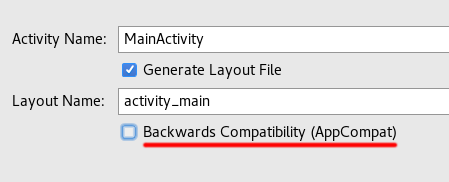
\includegraphics[scale=\SourceCodeScale]{chapters/ch12/images/1}
	\end{center}
	
	Run the project on a physical device and make sure it is working properly.
\end{enumerate}	

\subsection{Create an App on Facebook}
\label{FBI:createApponFacebook}
In order to connect your android app to facebook you need to create a corresponding app on the facebook site as well. This has to be done for every android app that you develop and wish to integrate with facebook. Let's do that!

Go to the \href{https://developers.facebook.com/}{facebook developer's portal} and register yourself as a developer. Usually this process is just a button click away. After you've done this locate drop down menu on the upper right corner named ``My Apps'' and click on "Add a New App":

\begin{center}
	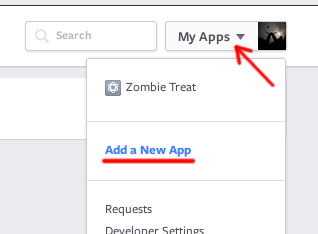
\includegraphics[scale=\SourceCodeScale]{chapters/ch12/images/2}
\end{center}

A dialog box will appear. Enter display name of your app as ``Test Application''. Note that the display name can be anything, it can be different from your android app. This is just for your reference. After that you must enter your email
address. Finally select the category that closely matches that of the android app which you wish to develop:

\begin{center}
	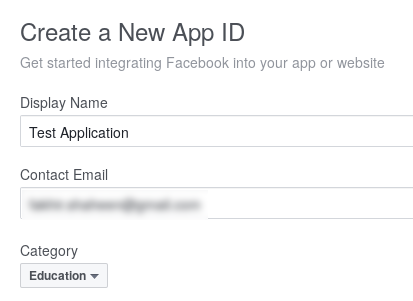
\includegraphics[scale=\SourceCodeScale]{chapters/ch12/images/3}
\end{center}

After you click on ``Create App ID'' button it will take you through a security check and finally create the app taking you to its dashboard. If you don't see the app dashboard then you can go to the facebook \href{https://developers.facebook.com/}{developer home page} and select your app from the drop down menu ``My Apps'' located in the top right corner.

Once you've opened the dashboard, go to the panel at the left side and then select ``Settings $\rightarrow$ Basic'':

\begin{center}
	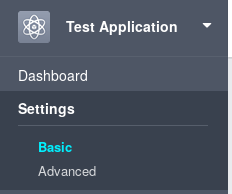
\includegraphics[scale=\SourceCodeScale]{chapters/ch12/images/4}
\end{center}

The basic settings will show up at the right side. Now we need to specify the platform (can be many) which our app will run onto. Near the bottom of the page you will see a ``Add Platform'' button:

\begin{center}
	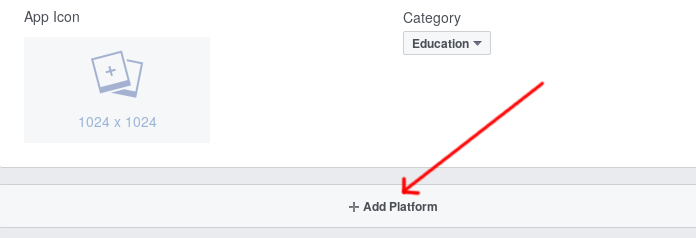
\includegraphics[scale=\SourceCodeScale]{chapters/ch12/images/5}
\end{center}

Click on it, this will open up a dialog box listing possible platforms that your app can support. Click on the android icon to add support for android. 

\begin{quote}
	\textit{``Tip: If you are developing your app for multiple platforms then you can set all of these up from here.''}
\end{quote}

A new panel for the android platform will appear near the bottom of the page. In the package name specify the package of your app. In our case it is ``\texttt{pk.edu.fccollege.madbookapp}''. In the class name you need to give the name of the main activity appended with the package name. In this case we give \texttt{pk.edu.fccollege.madbookapp.MainActivity}. Also there is a button named "Single Sign On" near the bottom, switch it to ``On'' state:

\begin{center}
	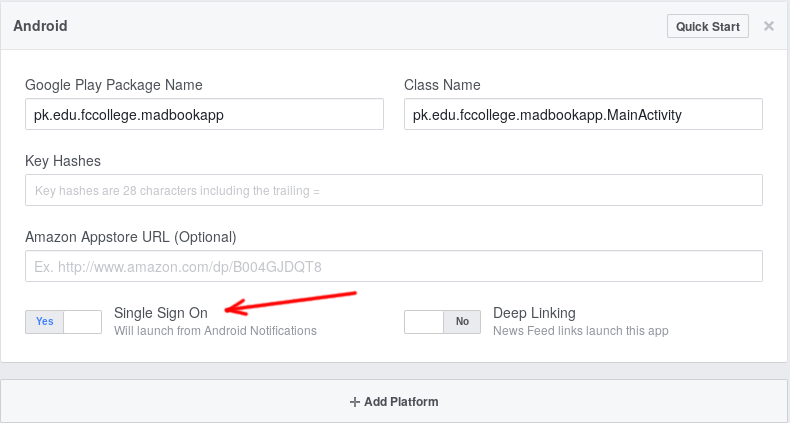
\includegraphics[scale=\SourceCodeScale]{chapters/ch12/images/6}
\end{center}

Finally we need the missing piece of the puzzle, the key hashes. For windows you need to execute ``\texttt{keytool.exe}'' which is located in the ``\texttt{<JDK-path>\\bin}'' folder. If you've setup jdk paths in the system environment then you should be able to run \texttt{keytool.exe} from anywhere. Second thing you'll need to install is the \texttt{openssl}. Just follow \href{https://sourceforge.net/projects/openssl/}{this} link, download and install \texttt{openssl}. You can add it to the system path so that \texttt{openssl} command can be executed from anywhere. Finally from the command prompt run the following (the following command is in single line, we are writing here in multiple lines due to limited space): 

\begin{verbatim}
c:\> keytool -exportcert -alias androiddebugkey -keystore
              %HOMEPATH%\.android\debug.keystore 
              | openssl sha1 -binary | openssl base64
\end{verbatim}

This will ask you for a password. Give it anything reasonable. Finally the utility will output a ``key hash'' string that we need:

\begin{center}
	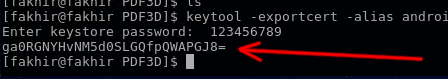
\includegraphics[scale=\SourceCodeScale]{chapters/ch12/images/7}
\end{center}

Copy this string and paste in the ``Key Hashes'' field located within the android panel in the app dashboard:

\begin{center}
	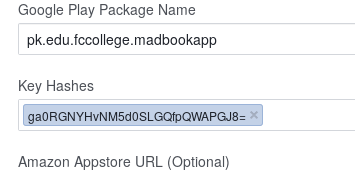
\includegraphics[scale=\SourceCodeScale]{chapters/ch12/images/8}
\end{center}

Finally hit the ``Save Changes'' button located at the lower right corner, a warning dialog box will show up asking you that your app is not on the appstore yet do you want to proceed. Just click ``Use this package name'' button to finalize the settings.

\section{Prepare Android Project}

Open up your facebook app's dashboard. From the panel at the left select ``Settings $\rightarrow$ Basic''. Note down the \texttt{App Id}, we'll be needing it very soon:

\begin{center}
	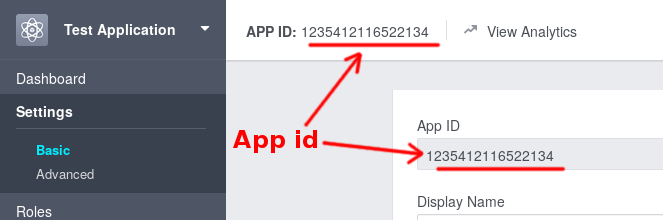
\includegraphics[scale=\SourceCodeScale]{chapters/ch12/images/9}
\end{center}

Great, now open up the project that we created earlier in section \ref{FBI:createProj}. Add the following line (line 3) in \texttt{strings.xml} file. It specifies the app id that we just copied from the dashboard:

\begin{center}
	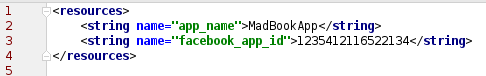
\includegraphics[scale=\SourceCodeScale]{chapters/ch12/images/10}
\end{center}

Now we need to setup the actual facebook sdk. Go to the project panel, switch to ``android'' mode. Open up \texttt{build.gradle(Module:app)} file (Do not open the wrong gradle file):

\begin{center}
	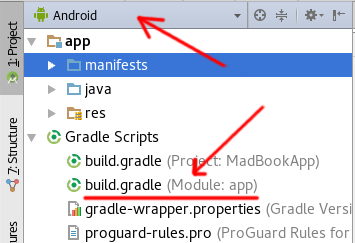
\includegraphics[scale=\SourceCodeScale]{chapters/ch12/images/12}
\end{center}

Add maven repository in build.gradle file (lines 22 to 24). Maven repositories are basically an online server that holds a lot of repositories. You can search the database \href{http://search.maven.org/}{here}. These lines tell android studio where to fetch the facebook sdk. Next tell the android studio exactly which facebook sdk to link the project with (line 32). This was taken from the facebook's official documentation:

\begin{center}
	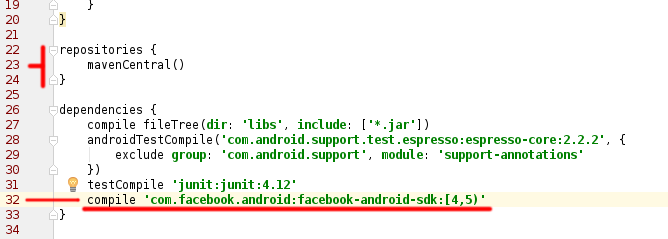
\includegraphics[scale=\SourceCodeScale]{chapters/ch12/images/13}
\end{center}

Note that we've just added the above code in \texttt{build.gradle} as shown above, we haven't deleted or modified anything else. Save the file and select ``Sync now'' option located in the upper right corner of the editor. It should sync successfully. But in case if you get any errors related to missing components, simply click and install those and it will sync successfully:

\begin{center}
	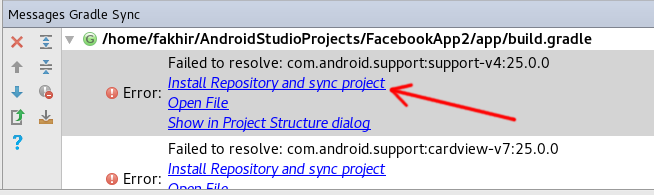
\includegraphics[scale=\SourceCodeScale]{chapters/ch12/images/14}
\end{center}

Open up \texttt{AndroidManifest.xml} file. Add a meta-data tag INSIDE the \texttt{<application>} tag but OUTSIDE any \texttt{<activity>} tags as shown below (in lines 19 and 20). Also add internet permission OUTSIDE the \texttt{<application>} tag (line 24):

\begin{center}
	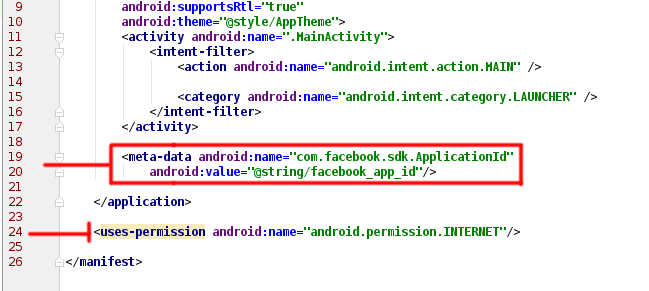
\includegraphics[scale=\SourceCodeScale]{chapters/ch12/images/11}
\end{center}

To use facebook api in your android app you must also add a facebook activity in the manifest file as shown below. This code has been taken from official facebook documentation so you should be able to copy it into your project without any change (lines 19 to 23):

\begin{center}
	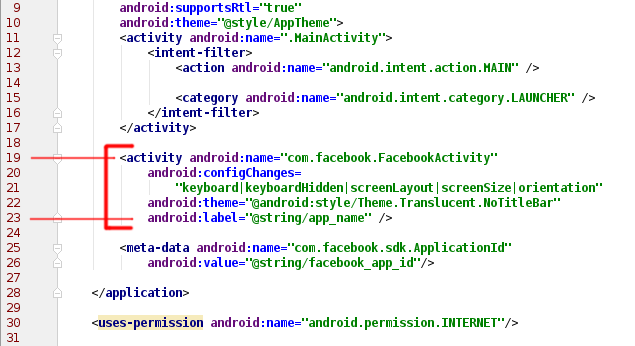
\includegraphics[scale=\SourceCodeScale]{chapters/ch12/images/15}
\end{center}

At this point if you've followed all the steps correctly there should be no error. Open up \texttt{MainActivity.java} and add the following code inside the \texttt{onCreate} method (lines 14 and 15):

\begin{center}
	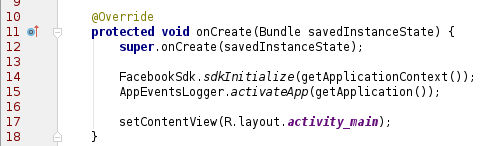
\includegraphics[scale=\SourceCodeScale]{chapters/ch12/images/16}
\end{center}

Code explanation:
\begin{itemize}
	\item \textit{Line 14:} This initializes the facebook sdk. For further reference you can read \href{https://developers.facebook.com/docs/reference/android/current/class/FacebookSdk/}{here}.
	
	\textbf{IMPORTANT:} Facebook sdk MUST be initialized before displaying the activity layout. This is why this call is placed BEFORE \texttt{setContentView}.
	
	\item \textit{Line 15:} Initialize the event logger. With the event logger you can track how the user is using your app, which activities is he running most frequently, how many times per day he logs in, how many friends he tagged in past 5 hours etc. You can read more about event logger \href{https://developers.facebook.com/docs/reference/android/current/class/AppEventsLogger/}{here}.
\end{itemize}

At this point if you run the app on a device you may (or may not) get theme conflict related errors as follows:

\begin{center}
	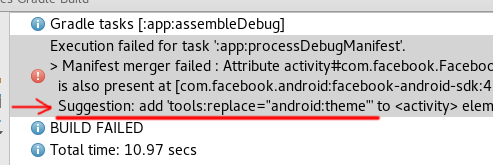
\includegraphics[scale=\SourceCodeScale]{chapters/ch12/images/17}
\end{center}

Don't worry, this is very easy to fix. As suggested in the error itself, open up \texttt{AndroidManifest.xml} and add \texttt{tools:replace} attribute inside the facebook activity as shown below (line 24):

\begin{center}
	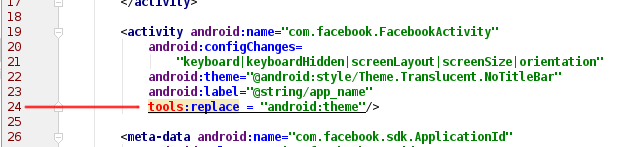
\includegraphics[scale=\SourceCodeScale]{chapters/ch12/images/18}
\end{center}

Finally either bring keyboard cursor on top of the red colored ``tools'' keyword. Android studio should show a tool tip asking you to press ``\texttt{Alt+Enter}'' to add a tools namespace definition. Alternatively you can manually add the namespace definition as an attribute in the \texttt{<manifest>} tag as shown below (line 3):

\begin{center}
	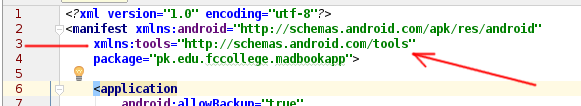
\includegraphics[scale=\SourceCodeScale]{chapters/ch12/images/19}
\end{center}

If you've followed all the steps correctly you should be able to run the app on a device without any errors at all.

\section{Facebook Login}

\subsection{Setting up Login Button}
The simplest way to add login functionality is through the facebook button. Open \texttt{activity\_main.xml} in text mode and add replace it with the following code (note we deleted the default text view):

\begin{center}
	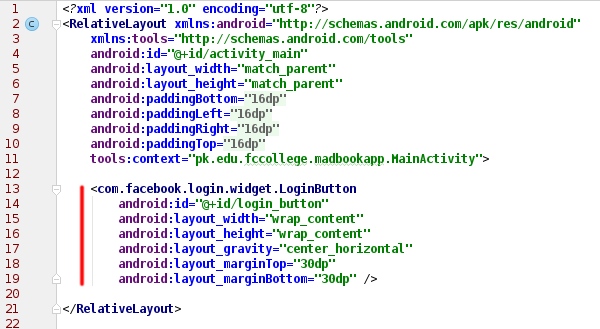
\includegraphics[scale=\SourceCodeScale]{chapters/ch12/images/20}
\end{center}

Switch to design mode and you should see a facebook login button:

\begin{center}
	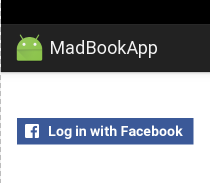
\includegraphics[scale=\SourceCodeScale]{chapters/ch12/images/21}
\end{center}

If you run the app on a device and press the login button, it will ask you for permissions which you should allow. 

A rare chance but you app can generate an error saying ``invalid hash key'':

\begin{center}
	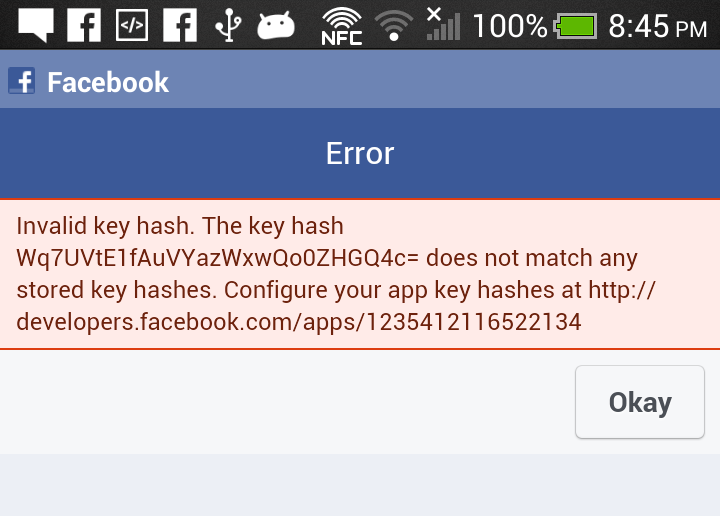
\includegraphics[scale=0.20]{chapters/ch12/images/22}
\end{center}

This is also pretty easy to fix. Complete solution is given \href{http://stackoverflow.com/questions/23674131/android-facebook-integration-invalid-key-hash}{here}. \\

We need to do a few more things before we can finally login successfully. According to facebook documentation you must override \texttt{onActivityResult} method. Open up \texttt{MainActivity.java} and create a member variable of type \texttt{CallbackManager} (line 13):

\begin{center}
	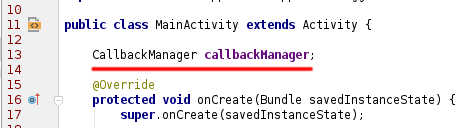
\includegraphics[scale=\SourceCodeScale]{chapters/ch12/images/23}
\end{center}

\texttt{CallbackManager} is responsible for gluing together the facebook sdk and the activity. We must initialize it inside \texttt{onCreate} method as shown:

\begin{center}
	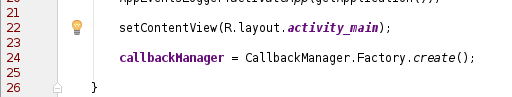
\includegraphics[scale=\SourceCodeScale]{chapters/ch12/images/24}
\end{center}

And we also need to override \texttt{MainActivity}'s \texttt{onActivityResult} and implement it as shown below. The following code was taken from official facebook documentation. It is almost identical for all android projects:

\begin{center}
	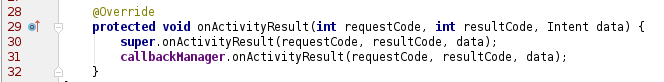
\includegraphics[scale=\SourceCodeScale]{chapters/ch12/images/25}
\end{center}

Now when you run the app on a device you should be finally able to login and logout of the facebook. Facebook button will actually change depending on your current status. This is functional but a bit boring. Let's make it interesting.

\subsection{Handling Login Callbacks}
We need to know whether the login was successful or did it fail. For that we need to attach callback methods to the facebook\texttt{LoginManager}. Inside the \texttt{onCreate} method, right after initializing the \texttt{callbackManager} object add the following code to register the login event handlers (lines 30 to 46):

\begin{center}
	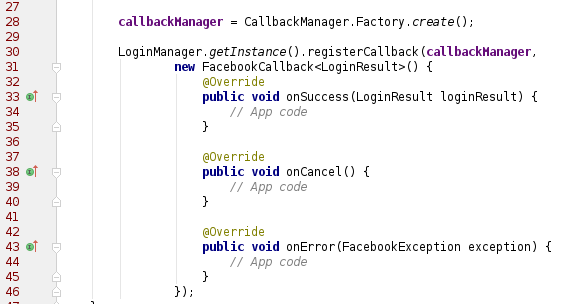
\includegraphics[scale=\SourceCodeScale]{chapters/ch12/images/26}
\end{center}

Code explanation:
\begin{itemize}
	\item \textit{Lines 30 to 31:} This code should seem familiar by now. We've been doing it to attach event handlers to buttons, widgets etc. 
	
	\item \textit{Lines 32 to 35:} When the user successfully logs in the \texttt{onSuccess} method will be called.
	
	\item \textit{Lines 37 to 40:} Login process was canceled.
	
	\item \textit{Lines 42 to 45:} Login process was failed, such as invalid user credentials.
	
\end{itemize}

\subsection{Exercise 1}
\label{FBI:exercise1}
Open up \texttt{activity\_main.xml} layout file. Add a text view and a button (initially disabled) underneath the facebook button. Whenever login is successful the text view should display ``Login Successful!!'' and the button gets enabled. It should display appropriate messages for other login callback methods and disable the proceed button. The ``proceed'' button does nothing for now but later on we will call another activity from it.

\begin{center}
	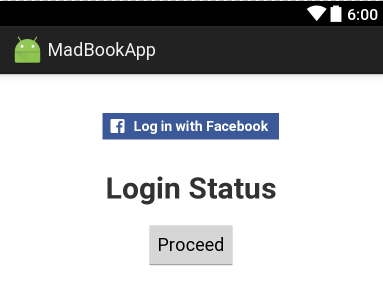
\includegraphics[scale=\SourceCodeScale]{chapters/ch12/images/27}
\end{center}

\textbf{Question:} 

What is an \textit{Access Token}? Hints \href{https://developers.facebook.com/docs/facebook-login/access-tokens/}{here} and \href{https://developers.facebook.com/docs/marketing-api/authentication}{here}.

\subsection{Exercise 2}
\label{FBI:exercise2}
Sometimes when you run the app it is already logged in, the facebook button with actually show ``Log Out'' message. In this case it will NOT go into the callback methods, so our text view and button will not properly get updated. Fix this issue. Check at the beginning of the activity whether if the user is already logged in or not. If the user is already logged in then update the UI immediately.

\textit{Hint:} \href{http://stackoverflow.com/questions/29294015/how-to-check-if-user-is-logged-in-with-fb-sdk-4-0-for-android}{here}.

\subsection{Exercise 3}
\label{FBI:exercise3}
Right now the facebook button implements logout. But you need to register callbacks to detect whether the user has logged out and change the user interface (text view and button) accordingly.

\textit{Hint:} \href{http://stackoverflow.com/questions/29305232/facebook-sdk-4-for-android-how-to-log-out-programmatically}{here}, \href{http://stackoverflow.com/questions/30360068/how-to-detect-logout-event-with-the-facebook-android-api-v4}{here} and \href{http://stackoverflow.com/questions/29294015/how-to-check-if-user-is-logged-in-with-fb-sdk-4-0-for-android}{here}.

\section{Access Personal Information}
\label{FBI:accessPersonalInformation}

Create a new activity named ``\texttt{PersonalActivity}'' and uncheck its backward compatibility check box. Leave all other options as default:

\begin{center}
	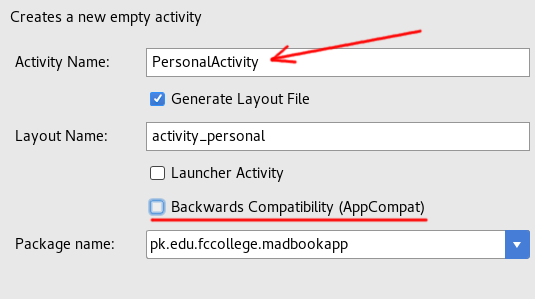
\includegraphics[scale=\SourceCodeScale]{chapters/ch12/images/28}
\end{center}

After creating the activity open up \texttt{MainActivity.java} and attach an event handler to the ``Proceed'' button. When this button is clicked it launches ``PersonalActivity''. Remepber that the proceed button will become enabled only if the user is successfully logged in:

\begin{center}
	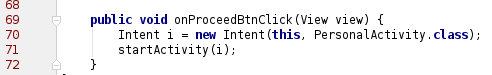
\includegraphics[scale=\SourceCodeScale]{chapters/ch12/images/29}
\end{center}

Run your app and make sure it is working properly. \\

Whenever we want to access some data or information from facebook we need to ask the user for permissions. Open up \texttt{MainActivity.java} and inside the \texttt{onCreate} method right after where you initialized facebook sdk add the following lines (31 to 45):

\begin{center}
	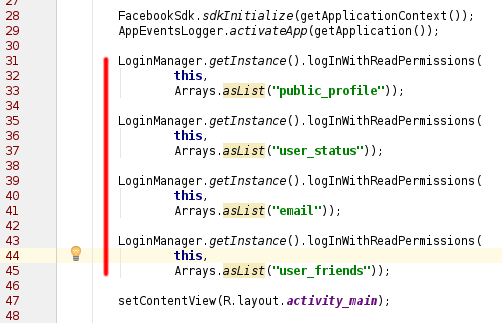
\includegraphics[scale=\SourceCodeScale]{chapters/ch12/images/30}
\end{center}

The code is simple. Here we are accessing four permissions i.e user's ``\textit{public profile}'', his ``\textit{facebook status}'', his ``\textit{email address}'' and his ``\textit{list of friends}''. \\

Open up \texttt{activity\_personal.xml} in text mode and add two things (lines ): 
\begin{enumerate}
	\item a text view
	\item a special widget called ``Profile Picture View''. Just add the following code inside root layout and it will display itself properly.
\end{enumerate}

\begin{center}
	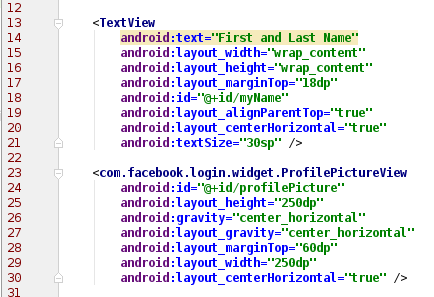
\includegraphics[scale=\SourceCodeScale]{chapters/ch12/images/31}
\end{center}

\texttt{activity\_personal.xml} looks like the following in design mode:

\begin{center}
	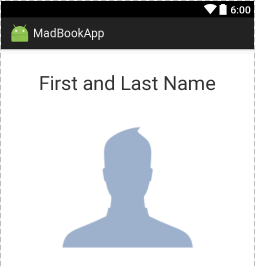
\includegraphics[scale=\FigureScale]{chapters/ch12/images/32}
\end{center}

\texttt{onCreate} method of \texttt{PersonalActivity}:

\begin{center}
	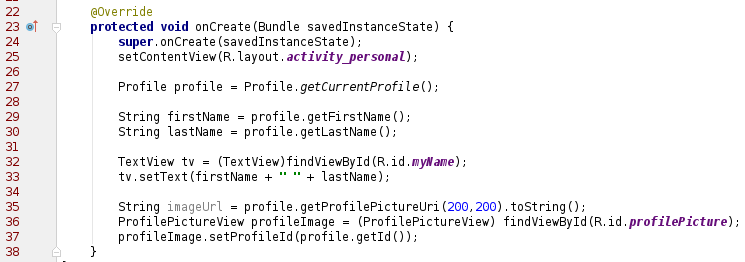
\includegraphics[scale=\SourceCodeScale]{chapters/ch12/images/33}
\end{center}


Run the app and it will display the name and the profile picture correctly:

\begin{center}
	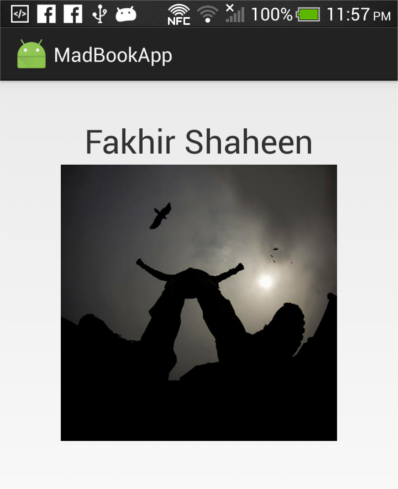
\includegraphics[scale=\FigureScale]{chapters/ch12/images/34}
\end{center}

\section{Sharing Content on Facebook}